Solange der Klotz ruht, ist die Reibungskraft eine Haftreibungskraft. Sie ist genau so gross wie die Zugkraft (Kräftegleichgewicht) und wächst mit ihr an. Sobald die Zugkraft den Höchstwert $\mu_\mathrm{H}\,F_\mathrm{N}$ erreicht, beginnt der Klotz zu rutschen. Von da an wirkt die Gleitreibungskraft $\mu_\mathrm{G}\,F_\mathrm{N}$, die kleiner ist und konstant bleibt, auch wenn die Zugkraft (gestrichelt) weiter zunimmt.

\begin{center}
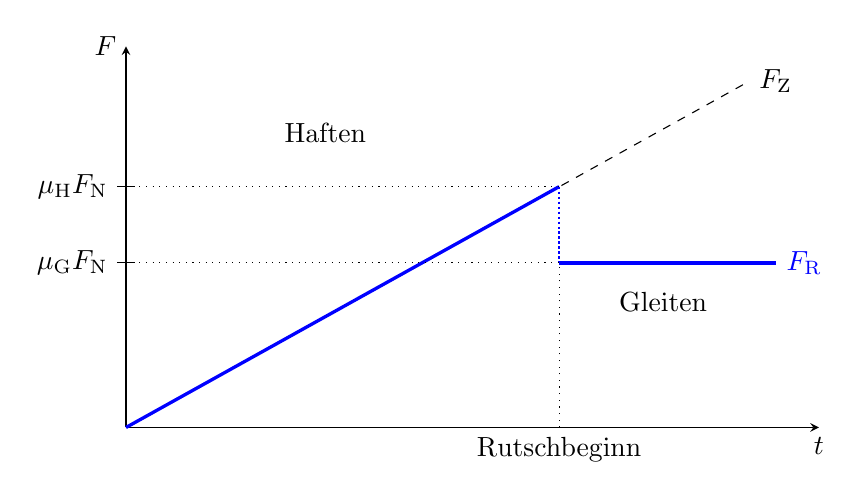
\begin{tikzpicture}[>=stealth, scale=1.1]
 \draw[->] (0,0) -- (8,0) node[below] {$t$};
 \draw[->] (0,0) -- (0,4.4) node[left] {$F$};
 \draw[dashed] (0,0) -- (7.2,4.0) node[right] {$F_\mathrm{Z}$};
 \draw[blue, very thick] (0,0) -- (5,2.78);
 \draw[blue, very thick] (5,1.9) -- (7.5,1.9) node[right] {$F_\mathrm{R}$};
 \draw[blue, thick, densely dotted] (5,2.78) -- (5,1.9);
 \draw (0.1,2.78) -- (-0.1,2.78) node[left] {$\mu_\mathrm{H}F_\mathrm{N}$};
 \draw (0.1,1.9) -- (-0.1,1.9) node[left] {$\mu_\mathrm{G}F_\mathrm{N}$};
 \draw[dotted] (0,2.78) -- (5,2.78);
 \draw[dotted] (0,1.9) -- (5,1.9);
 \draw[dotted] (5,0) -- (5,1.9);
 \node[below] at (5,0) {Rutschbeginn};
 \node at (2.3,3.4) {Haften};
 \node at (6.2,1.45) {Gleiten};
\end{tikzpicture}
\end{center}
Hier ist angenommen, dass die Zugkraft gleichmässig zunimmt.
